%----------------------------------------------------------------------------
% Synthetic example manuscript used to demonstrate the gate. The system,
% numbers, and references are invented. Replace with your own draft.
%----------------------------------------------------------------------------
\documentclass[conference]{IEEEtran}
\usepackage{graphicx}
\usepackage{booktabs}
\graphicspath{{figures/}}

\title{PebbleSort: Weight-Based Singulation of Small Parts on a Desktop Robot}
\author{Anonymous Submission}

\begin{document}
\maketitle

\begin{abstract}
Sorting small metal parts by weight is still done by hand in repair shops
because commercial sorters are sized for factories. We ask how much sorting
accuracy survives when the sorter is built from desktop components. PebbleSort
combines a hobby-grade arm, a load cell, and a scripted pick-weigh-place cycle.
Across 120 trials on two part families the system classifies 91\% of parts
correctly (95\% CI 85--95\%) at 40 parts per hour. Design files and trial logs
will be released.
\end{abstract}

\section{INTRODUCTION}
Repair shops receive mixed bins of fasteners that must be separated before
reuse. Industrial vibratory sorters solve the task at scale
\cite{doe2021sorters}, and learned tactile classifiers reach high accuracy on
laboratory arms \cite{roe2022tactile, lee2023grasp}. Neither fits on a shop
bench. The question this paper answers is how much accuracy survives when the
budget is cut by two orders of magnitude.

This paper contributes:
\begin{enumerate}
  \item a desktop sorter built from consumer components (Fig.~\ref{fig:system});
  \item a 120-trial characterization of accuracy and cycle time on two part
        families (Table~\ref{tab:results}).
\end{enumerate}

\section{SYSTEM}
\begin{figure}[t]
  \centering
  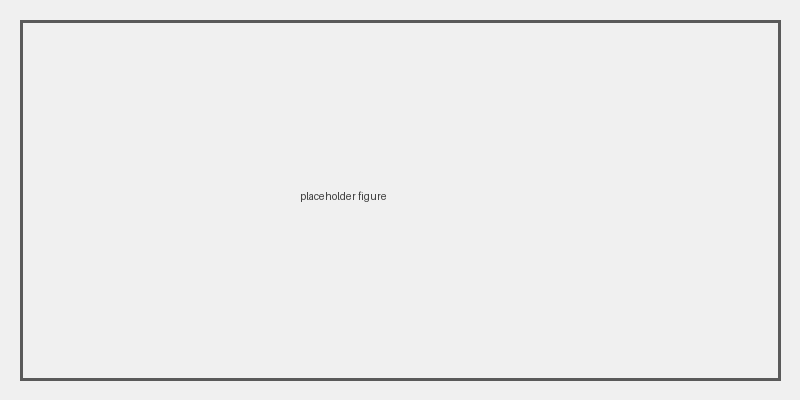
\includegraphics[width=\columnwidth]{placeholder.png}
  \caption{PebbleSort. Left: the arm above the input bin. Right: one
  pick-weigh-place cycle. The load cell reading decides the output bin.}
  \label{fig:system}
\end{figure}
The problem is distinguishing parts whose masses differ by under one gram.
A load cell with 0.1\,g resolution replaces vision, and a fixed dwell of 0.5\,s
lets the reading settle before classification.

\section{RESULTS}
\begin{table}[t]
  \caption{Results by part family (60 trials each).}
  \label{tab:results}
  \centering
  \begin{tabular}{@{}lcc@{}}
    \toprule
     & Screws & Washers \\
    \midrule
    Accuracy & 93.3\% (56/60) & 88.3\% (53/60) \\
    Cycle time, median (s) & 84 & 96 \\
    \bottomrule
  \end{tabular}
\end{table}
Both families sort reliably (Table~\ref{tab:results}). Washers are slower
because thin parts settle more slowly on the cell. The evidence indicates that
mass alone separates the two families at this resolution.

\section{LIMITATIONS}
The evaluation covers two part families and one operator. Parts lighter than
0.3\,g were not tested.

\section{CONCLUSION}
PebbleSort reaches 91\% sorting accuracy with desktop hardware. The next step
is a second load cell to remove the settling dwell.

\begin{thebibliography}{9}
\bibitem{doe2021sorters}
J.~Doe and A.~Smith, ``Vibratory sorting of fasteners: a survey,'' \emph{J.\
Manufacturing Systems}, vol.~12, no.~3, pp.~1--10, 2021.
\bibitem{roe2022tactile}
R.~Roe, ``Tactile classification of small parts,'' in \emph{Proc.\ Example
Conf.}, 2022, pp.~11--18.
\bibitem{lee2023grasp}
K.~Lee and M.~Park, ``Grasp-based part identification,'' in \emph{Proc.\
Example Conf.}, 2023, pp.~19--26.
\end{thebibliography}

\end{document}
